\documentclass[11pt]{article}
\usepackage[T1]{fontenc}
\usepackage[utf8]{inputenc}
\usepackage[portuguese]{babel}
\usepackage{amsmath}
\usepackage{graphicx}
\usepackage{float}
\usepackage{enumitem}

\graphicspath{{}}

\newcommand{\numpy}{{\tt numpy}}

\topmargin -.5in
\textheight 9in
\oddsidemargin -.25in
\evensidemargin -.25in
\textwidth 7in

\begin{document}

\author{Lucas Emanuel Resck Domingues}
\title{Aula prática 3
\medbreak
\large Métodos iterativos para cálculo de autovalores e autovetores}
\maketitle

\medskip

\begin{enumerate}

\item A função Scilab foi implementada e está presente no arquivo \textit{Functions.sce} anexado.

\item Idem.

\item Idem.

\item As funções foram testadas variando as variáveis de entrada, inclusive a matriz $A$ e sua ordem $n$. Alguns exemplos:

\begin{figure}[H]
    \centering
    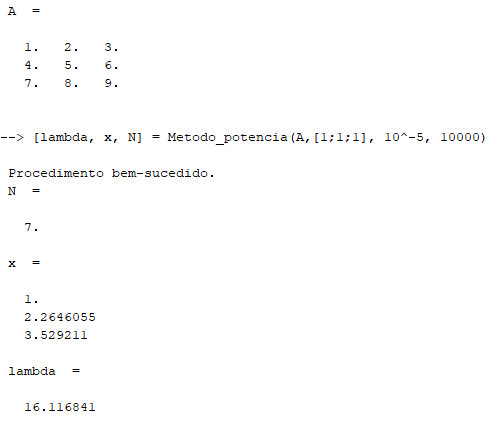
\includegraphics[]{4-1}
    \caption{Método da potência. Os resultados foram verificados.}
\end{figure}

\begin{figure}[H]
    \centering
    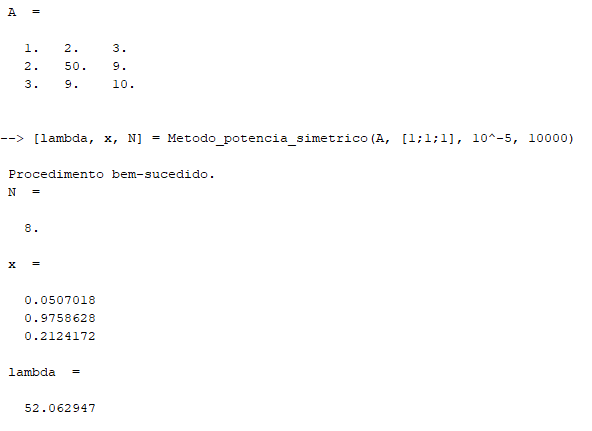
\includegraphics[]{4-2}
    \caption{Método da potência simétrico.}
\end{figure}

\begin{figure}[H]
    \centering
    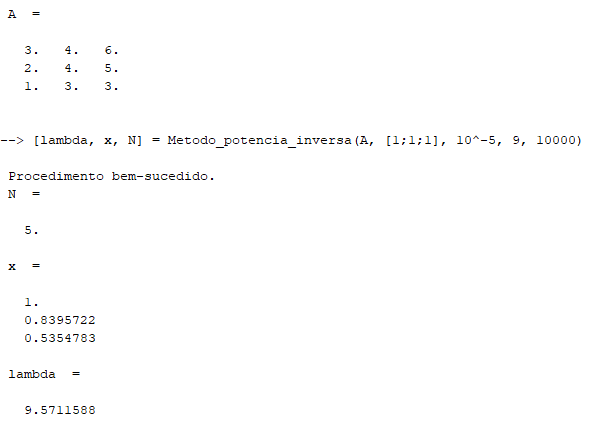
\includegraphics[]{4-3}
    \caption{Método da potência inversa.}
\end{figure}

Seja a matriz simétrica $A$:

$$A = \begin{bmatrix}
    9175& 5256& 19\\  
    5256& 8233& 82\\  
    19& 82& 6821
\end{bmatrix}$$

Vejamos como os algoritmos do método da potência e do método da potência simétrico se comportam e em quantas iterações eles resolvem o problema:

\begin{figure}[H]
    \centering
    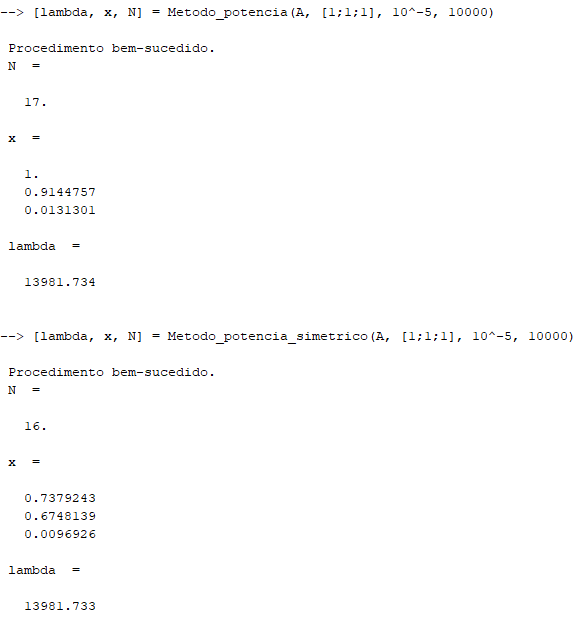
\includegraphics[]{4-4}
    \caption{Métodos da potência e da potência simétrico.}
\end{figure}

Neste caso o algoritmo do método da potência simétrico encontrou as aproximações em um número menor de iterações.

\item Pede-se para calcular $\rho(A^{-1})$, sendo $A_{10\times10}$:

$$A = \begin{bmatrix}
    1 + 2\alpha & -\alpha & 0& \ldots& 0\\
    -\alpha & 1 + 2\alpha & -\alpha & \ldots& 0\\
    0& -\alpha & 1 + 2\alpha & \ldots& 0\\
    \vdots &\vdots&\vdots & \ddots&\vdots\\
    0& 0& 0& \ldots& 1+2\alpha
\end{bmatrix}$$

Sabemos que $\rho(A^{-1})$ é o módulo do autovalor de maior módulo da matriz inversa de $A$, portanto o inverso do módulo do autovalor de menor módulo de $A$. Usamos $0$ como entrada para \textbf{alfa} no método da potência inversa para encontrar o módulo do autovalor de menor módulo de $A$.

\begin{enumerate}
    \item Para $\alpha = 1/4$, $\rho(A^{-1})\approx0,9801467$, então o método é estável.

\begin{figure}[H]
    \centering
    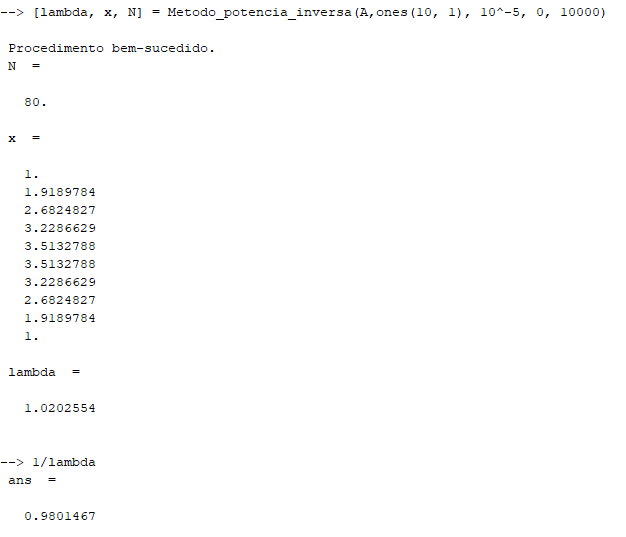
\includegraphics[]{5-a}
    \caption{Método da potência inversa.}
\end{figure}

    \item Para $\alpha = 1/2$, $\rho(A^{-1})\approx0,9610682$, então o método é estável.

\begin{figure}[H]
    \centering
    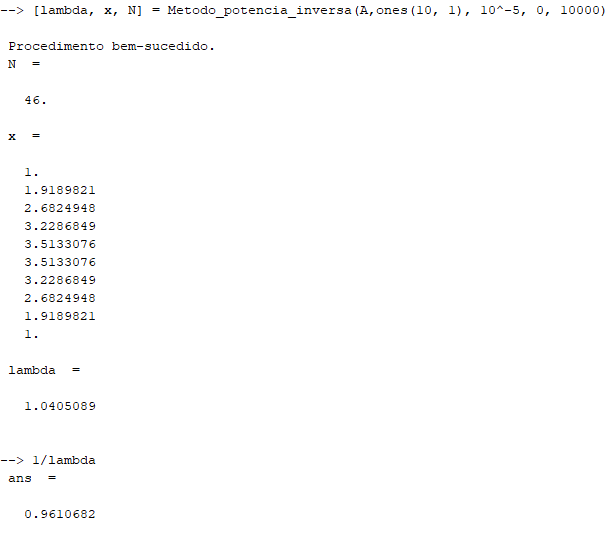
\includegraphics[]{5-b}
    \caption{Método da potência inversa.}
\end{figure}

    \item Para $\alpha = 3/4$, $\rho(A^{-1})\approx0,9427181$, então o método é estável.

\begin{figure}[H]
    \centering
    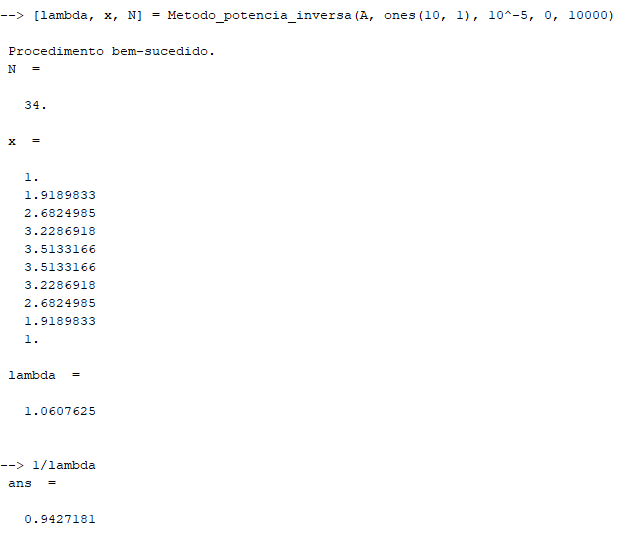
\includegraphics[]{5-c}
    \caption{Método da potência inversa.}
\end{figure}
\end{enumerate}

\end{enumerate}
\end{document}
\grid
\grid